% ============================================================
% Section 3: Data Specification & Experimental Protocol
% Target Journal: Neural Computing and Applications (Springer Nature)
% Scientific Audit (MISSION 11): Hedged scholarly phrasing applied.
% ============================================================

\section{Data Specification \& Experimental Protocol}\label{sec:data}

This section describes the high-frequency intraday financial dataset, the Information Gain feature selection methodology, and the sequential temporal validation protocol used across all optimizer evaluations.

\subsection{Intraday Mini-Index Futures Dataset}\label{sec:data_dataset}

The empirical evaluation is conducted on intraday price records of the Mini-Index futures contract (symbol: WIN), traded on B3 (Brazilian Stock Exchange). The dataset spans four consecutive quarterly contract maturities—WING24, WINJ24, WINM24, and WINQ24—sampled at a 5-minute bar frequency.

The complete dataset contains $N = 15,057$ clean, consecutive intraday instances. For each 5-minute bar, open, high, low, close (OHLC) prices, trading volume, and raw transaction indicators are recorded. The target variable is formulated as a binary trend classification label $y_k \in \{0, 1\}$ at bar index $k$:
\begin{equation}\label{eq:target}
    y_k = \begin{cases} 1 \quad (\text{Uptrend}) & \text{if } P_{k+1} > P_k \\ 0 \quad (\text{Downtrend}) & \text{if } P_{k+1} \le P_k \end{cases}
\end{equation}
where $P_k$ denotes the closing price at 5-minute bar $k$. Across the 15,057 total instances, the dataset exhibits a balanced target distribution of approximately 49.2\% uptrend ($y=1$) and 50.8\% downtrend ($y=0$) instances.

\subsection{Information Gain Feature Selection}\label{sec:data_features}

To mitigate dimensional overfitting while retaining informative technical market state signals, we apply Information Gain feature selection \cite{souza2025iccsa}. The initial feature candidate space consists of 66 technical indicators spanning trend-following moving averages, momentum oscillators, volatility bands, and volume indicators.

Information Gain measures the expected reduction in entropy $H(Y)$ resulting from observing feature $X_j$:
\begin{equation}\label{eq:infogain}
    I(Y; X_j) = H(Y) - H(Y \mid X_j) = \sum_{y \in Y} \sum_{x \in X_j} p(x, y) \log_2 \left( \frac{p(x, y)}{p(x) p(y)} \right)
\end{equation}

Based on ranking scores established in prior baseline research \cite{souza2025iccsa}, the top $d=7$ Information Gain features are selected to form the input feature vector $\boldsymbol{x}_k \in \mathbb{R}^7$. These seven attributes correspond to normalized technical indicators capturing multi-timeframe momentum and price dispersion relative to rolling moving averages.

\subsection{Sequential Temporal Validation Protocol}\label{sec:data_split}

A known limitation in published financial machine learning studies is the application of randomized $K$-fold cross-validation or unconstrained random sampling across time series \cite{souza2026ijcnn, makridakis2018statistical}. Shuffling intraday bars breaks chronological continuity, permitting future price information to contaminate historical training sets. This introduces look-ahead data leakage, producing validation metrics that fail to generalize under live market execution.

To prevent temporal look-ahead leakage within the adopted experimental design, we enforce a strict 60/20/20 sequential chronological split protocol with no shuffling (\texttt{shuffle = false}). The 15,057 intraday bars are partitioned sequentially along the time axis:
\begin{enumerate}
    \item \textbf{Training Set ($\mathcal{D}_{\text{train}}$)}: Consists of the first 60\% of chronological bars ($N_{\text{train}} = 9,034$ instances). Used exclusively for optimizing internal neural network connection weights during backpropagation.
    \item \textbf{Validation Set ($\mathcal{D}_{\text{val}}$)}: Consists of the subsequent 20\% of chronological bars ($N_{\text{val}} = 3,011$ instances). Used exclusively for evaluating optimizer candidate fitness $f(\boldsymbol{\theta})$ and triggering early stopping.
    \item \textbf{Out-of-Sample Test Set ($\mathcal{D}_{\text{test}}$)}: Consists of the final 20\% of chronological bars ($N_{\text{test}} = 3,012$ instances). Reserved strictly for evaluating out-of-sample classification metrics and financial backtesting.
\end{enumerate}

Figure~\ref{fig:temporal_split} illustrates the sequential temporal partitioning scheme, designed to maintain strict temporal ordering ($T_{\text{train}} < T_{\text{val}} < T_{\text{test}}$) across all evaluation stages.

\begin{figure}[htbp]
\centering
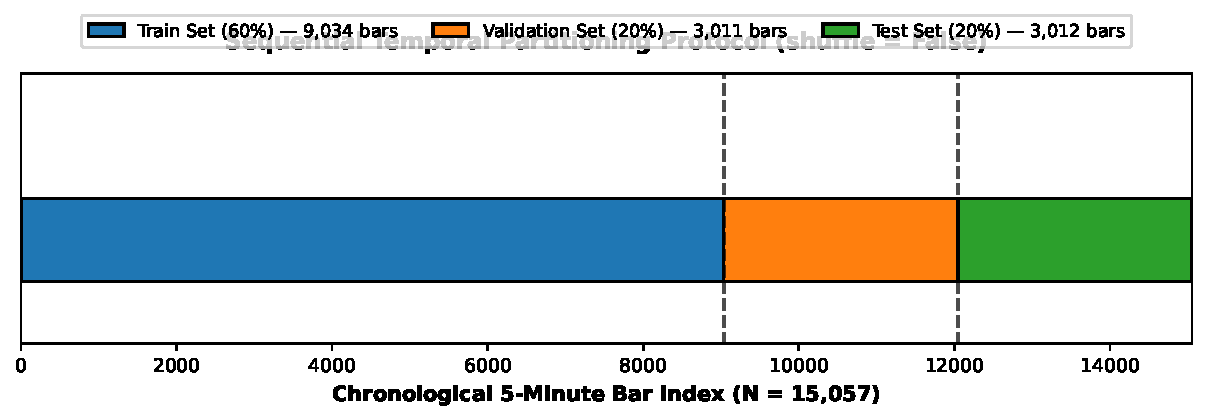
\includegraphics[width=0.85\linewidth]{figures/temporal_split.pdf}
\caption{Chronological 60/20/20 sequential temporal partitioning protocol ($N = 15,057$ 5-minute bars) designed to preserve temporal ordering ($T_{\text{train}} < T_{\text{val}} < T_{\text{test}}$) and preclude look-ahead data leakage.}
\label{fig:temporal_split}
\end{figure}
